\documentclass{beamer}
\usepackage{graphicx}
\usepackage{kotex}

\usetheme{Berlin}

\title{JetBrains 학생용 라이센스 인증하기}
\author{허강준}
\institute{충남대학교 정보보호동아리 ARGOS}
\date{2021. 03. 23}

\begin{document}

\begin{frame}
    \begin{center}
        
\includegraphics[height=1.5cm]{../Images/logo.png}
    \end{center}

    \maketitle
\end{frame}

\section{JetBrains 소개}
    \begin{frame}{JetBrains?}
        \begin{itemize}
            \item 개발도구 및 언어 개발회사
            \item IntelliJ IDEA, Android Studio 개발
            \item 기본적으로 유료 프로그램들이지만
            \item 학생 인증시 전 제품 1년 사용 가능!
        \end{itemize}
    \end{frame}

    \begin{frame}{JetBrains?}
        전부 무료로 사용 가능!
        \begin{columns}
            \begin{column}{0.45\textwidth}
                \begin{itemize}
                    \item IntelliJ: Java, Kotlin..
                    \item CLion: C/C++
                    \item DataGrip: SQL
                    \item GoLand: Go
                \end{itemize}
            \end{column}
            \begin{column}{0.55\textwidth}
                \begin{itemize}
                    \item Rider: .NET
                    \item RubyMine: Ruby
                    \item WebStorm: Java(Type)Script
                    \item AppCode: ObjC, Swift..
                \end{itemize}
            \end{column}
        \end{columns}
    \end{frame}

\section{학생용 라이센스 활성화하기}
    \begin{frame}
        \begin{itemize}
            \item https://www.jetbrains.com/community/education
        \end{itemize}
        \begin{center}
            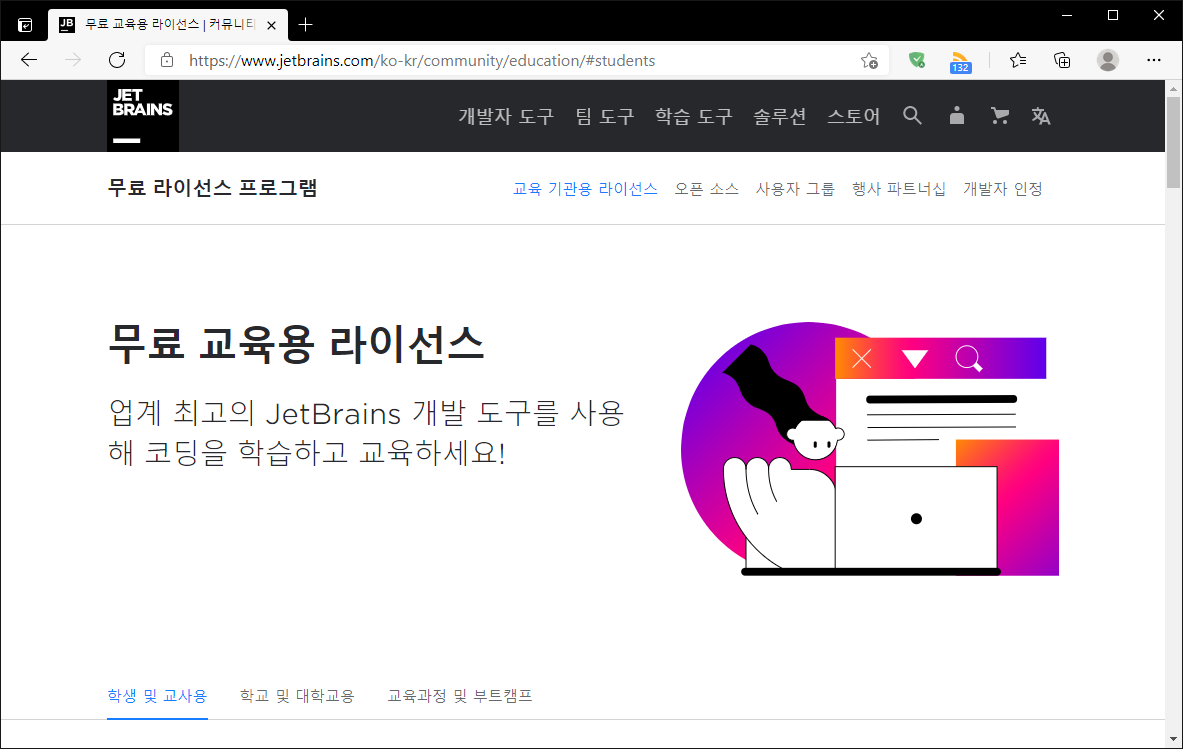
\includegraphics[height=5cm]{Images/jetbrains-1.png}
        \end{center}
    \end{frame}
    \begin{frame}
        \begin{itemize}
            \item {[지금 신청하기]} 클릭
        \end{itemize}
        \begin{center}
            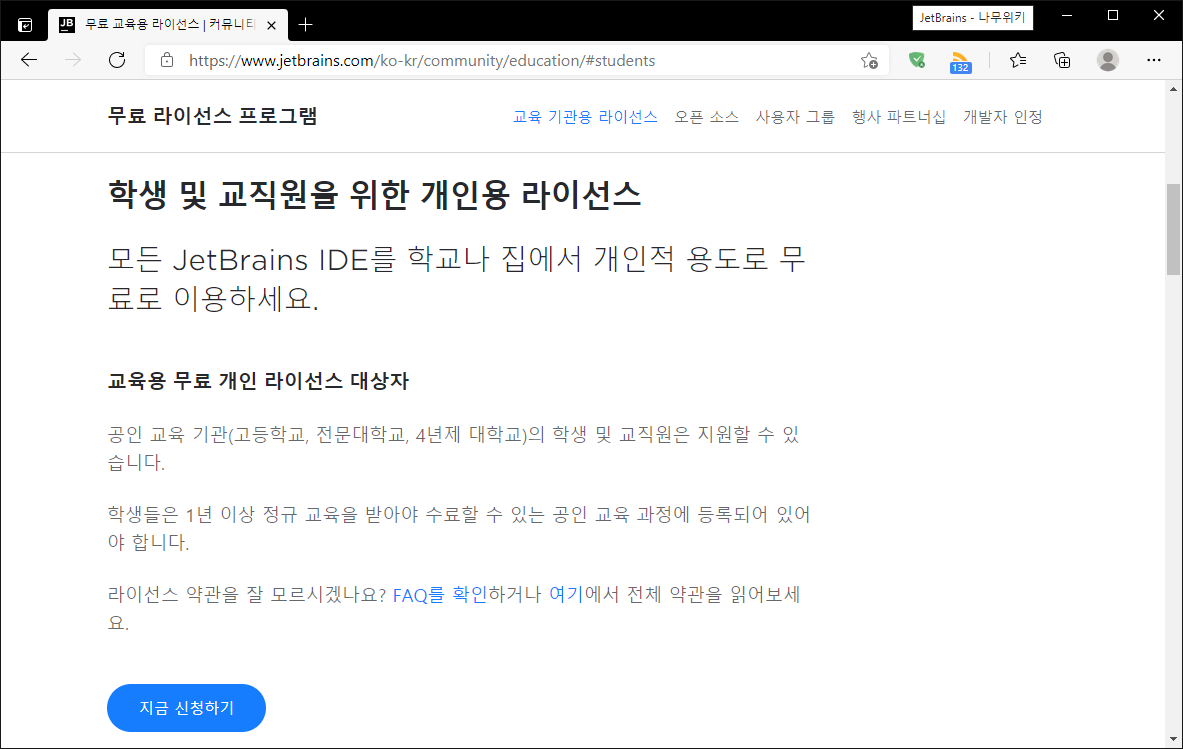
\includegraphics[height=5cm]{Images/jetbrains-2.png}
        \end{center}
    \end{frame}
    \begin{frame}
        \begin{itemize}
            \item 관련 정보(학교 메일 필수) 전부 입력하고...
        \end{itemize}
        \begin{center}
            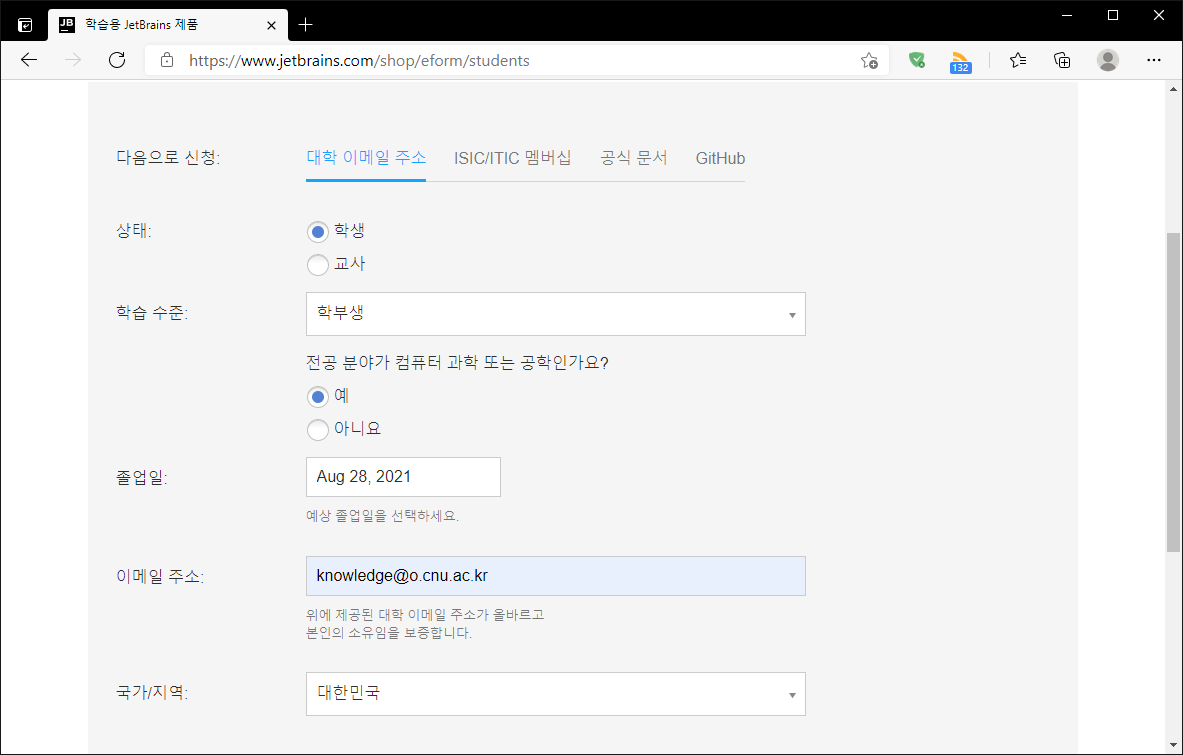
\includegraphics[height=5cm]{Images/jetbrains-3.png}
        \end{center}
    \end{frame}
    \begin{frame}
        \begin{itemize}
            \item {[무료 제품 신청]} 클릭
        \end{itemize}
        \begin{center}
            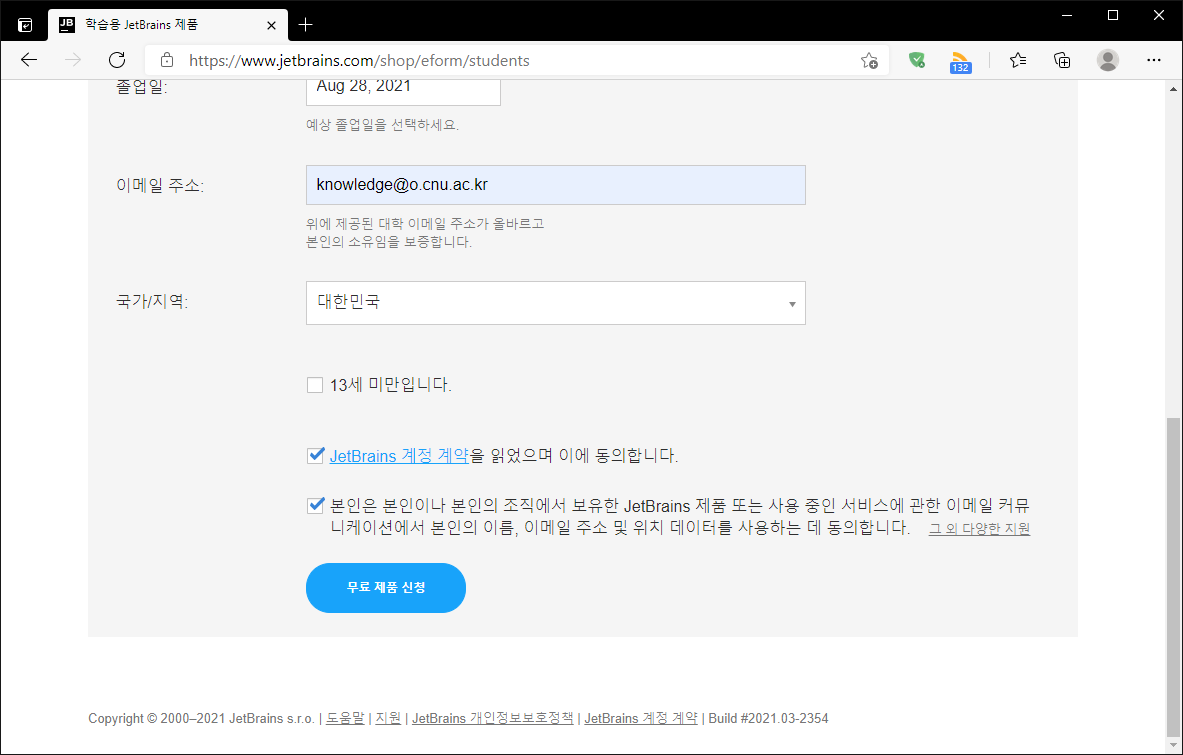
\includegraphics[height=5cm]{Images/jetbrains-5.png}
        \end{center}
    \end{frame}
    \begin{frame}
        \begin{itemize}
            \item 메일함 확인하기
        \end{itemize}
        \begin{center}
            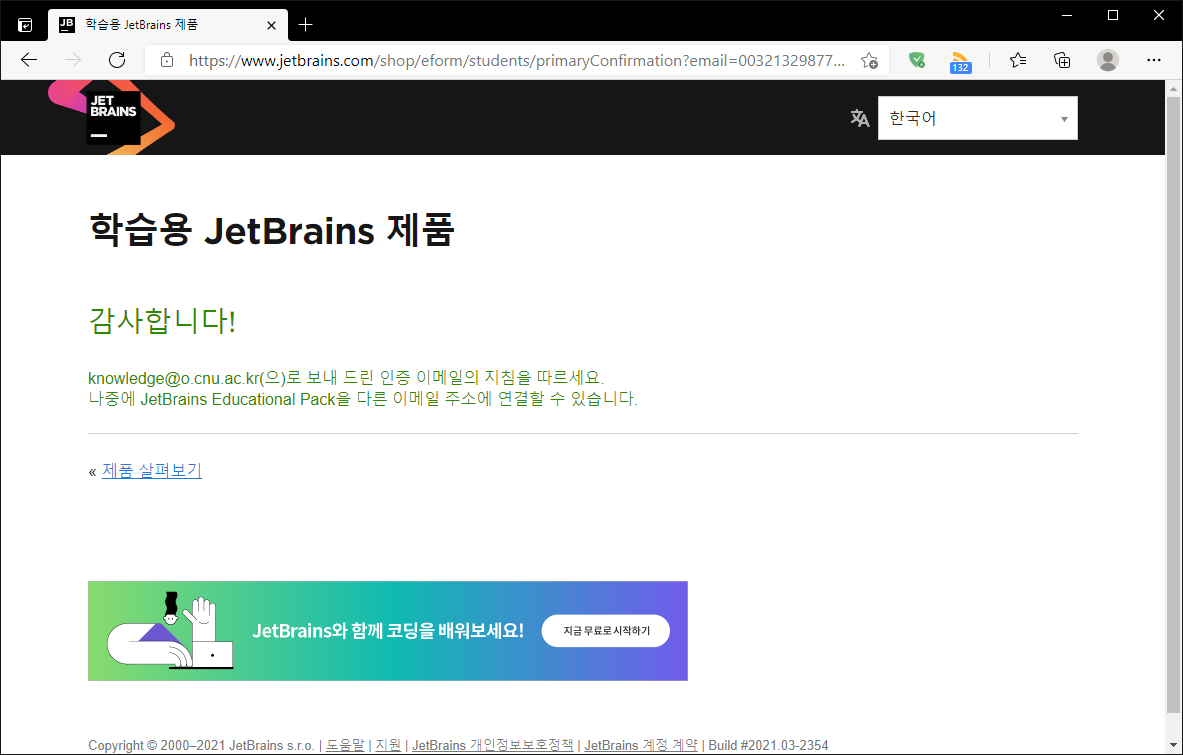
\includegraphics[height=5cm]{Images/jetbrains-6.png}
        \end{center}
    \end{frame}
    \begin{frame}
        \begin{itemize}
            \item 링크 클릭하기 (없으면 스팸함 확인!)
        \end{itemize}
        \begin{center}
            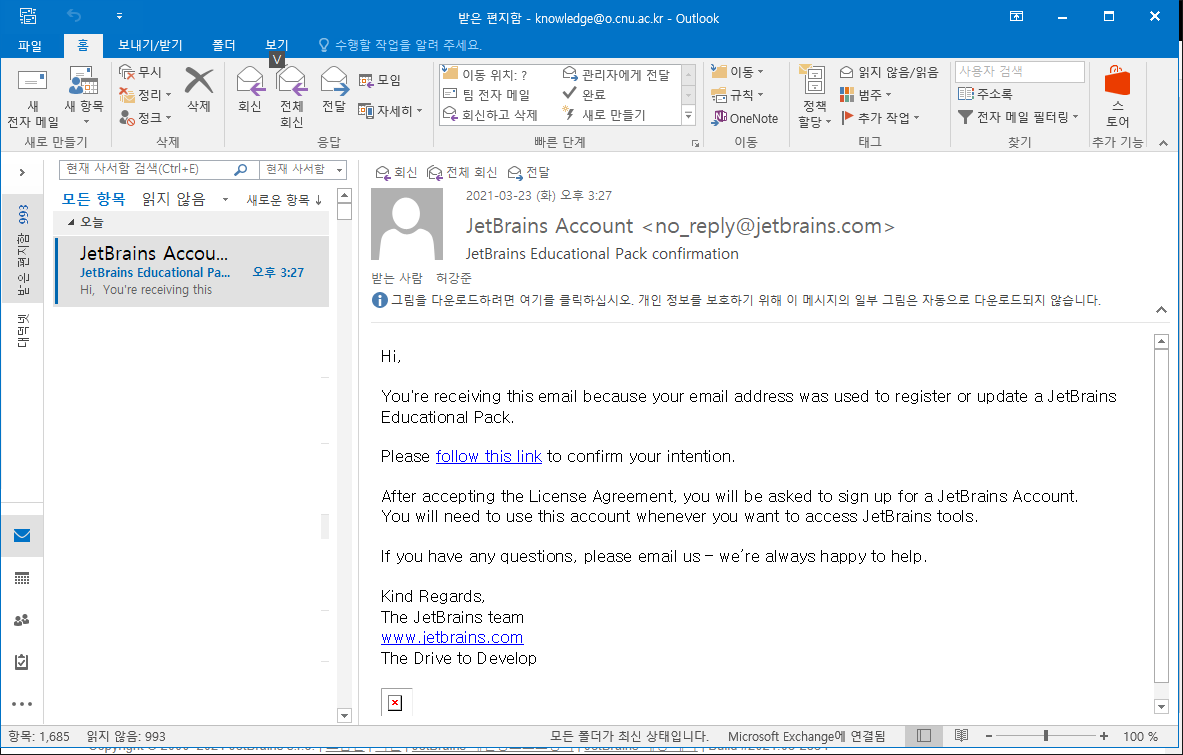
\includegraphics[height=5cm]{Images/jetbrains-7.png}
        \end{center}
    \end{frame}
    \begin{frame}
        \begin{itemize}
            \item JetBrains 계정 가입하기 (나중에 필요)
        \end{itemize}
        \begin{center}
            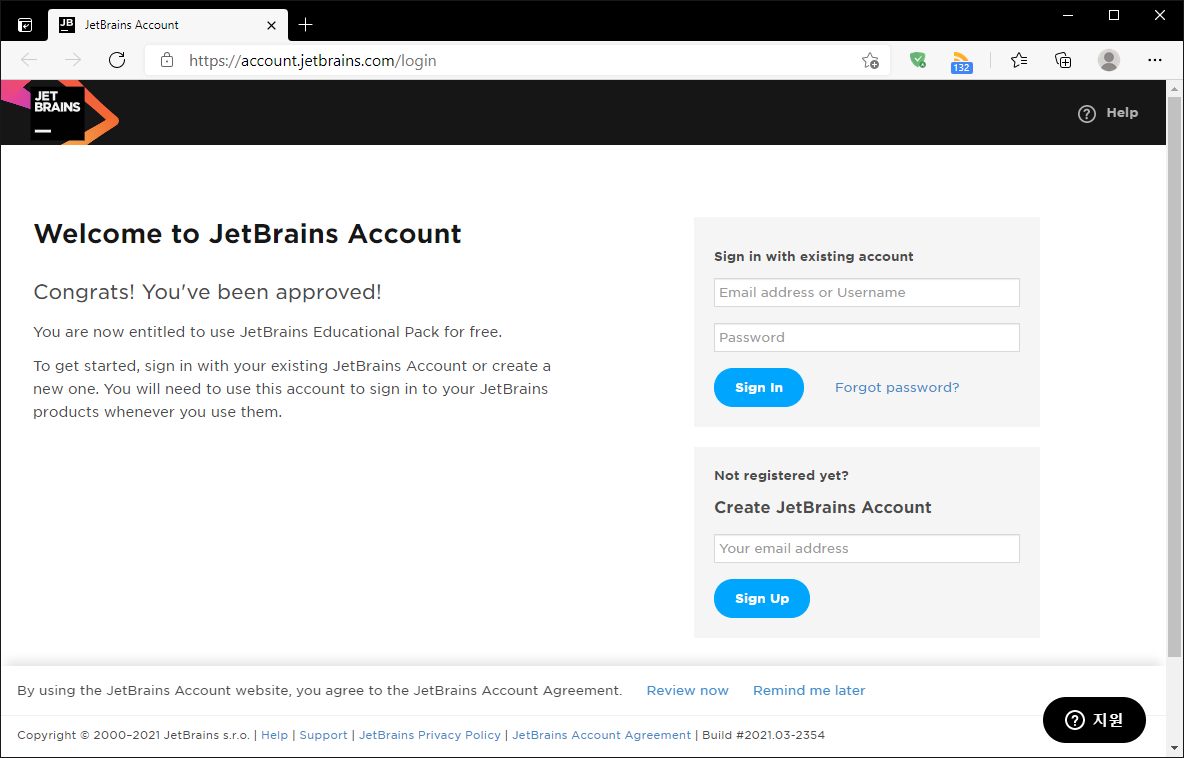
\includegraphics[height=5cm]{Images/jetbrains-8.png}
        \end{center}
    \end{frame}
\section{정리하기}
    \begin{frame}{JetBrains 계정에 가입해야 하는 이유}
        \begin{itemize}
            \item 학생용 라이센스 연장할 때 필요
            \item 프로그램 정품인증 할 때도 필요 (중요)
        \end{itemize}
    \end{frame}
    \begin{frame}
        \begin{itemize}
            \item 나중에 프로그램 실행할 때 정품인증 창에서 사용
        \end{itemize}
        \begin{center}
            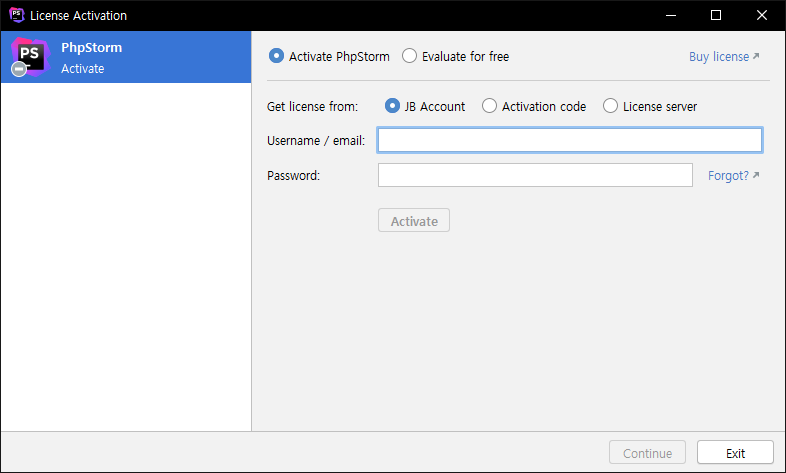
\includegraphics[height=5cm]{Images/jetbrains-9.png}
        \end{center}
    \end{frame}
    \begin{frame}{질문이 있는 경우...}
        \begin{center}
            자료 레포지토리의 이슈트래커에 이슈를 남겨주세요!
        \end{center}
    \end{frame}
\end{document}